\section{Humanoid Walking}
\label{sec::31_hw}
To get started with and to understand the presented concepts that generate dynamically balanced walking trajectories, we shall have a look at figure \ref{fig::3_cl} once more. The pattern generation therein (orange box), consists of four main building blocks: Forward kinematics, nonlinear model predictive control (NMPC), interpolation, and inverse kinematics. The relation between these four building blocks is shown in fig. \ref{fig::31_pg}.
\begin{figure}[h]
	\centering
	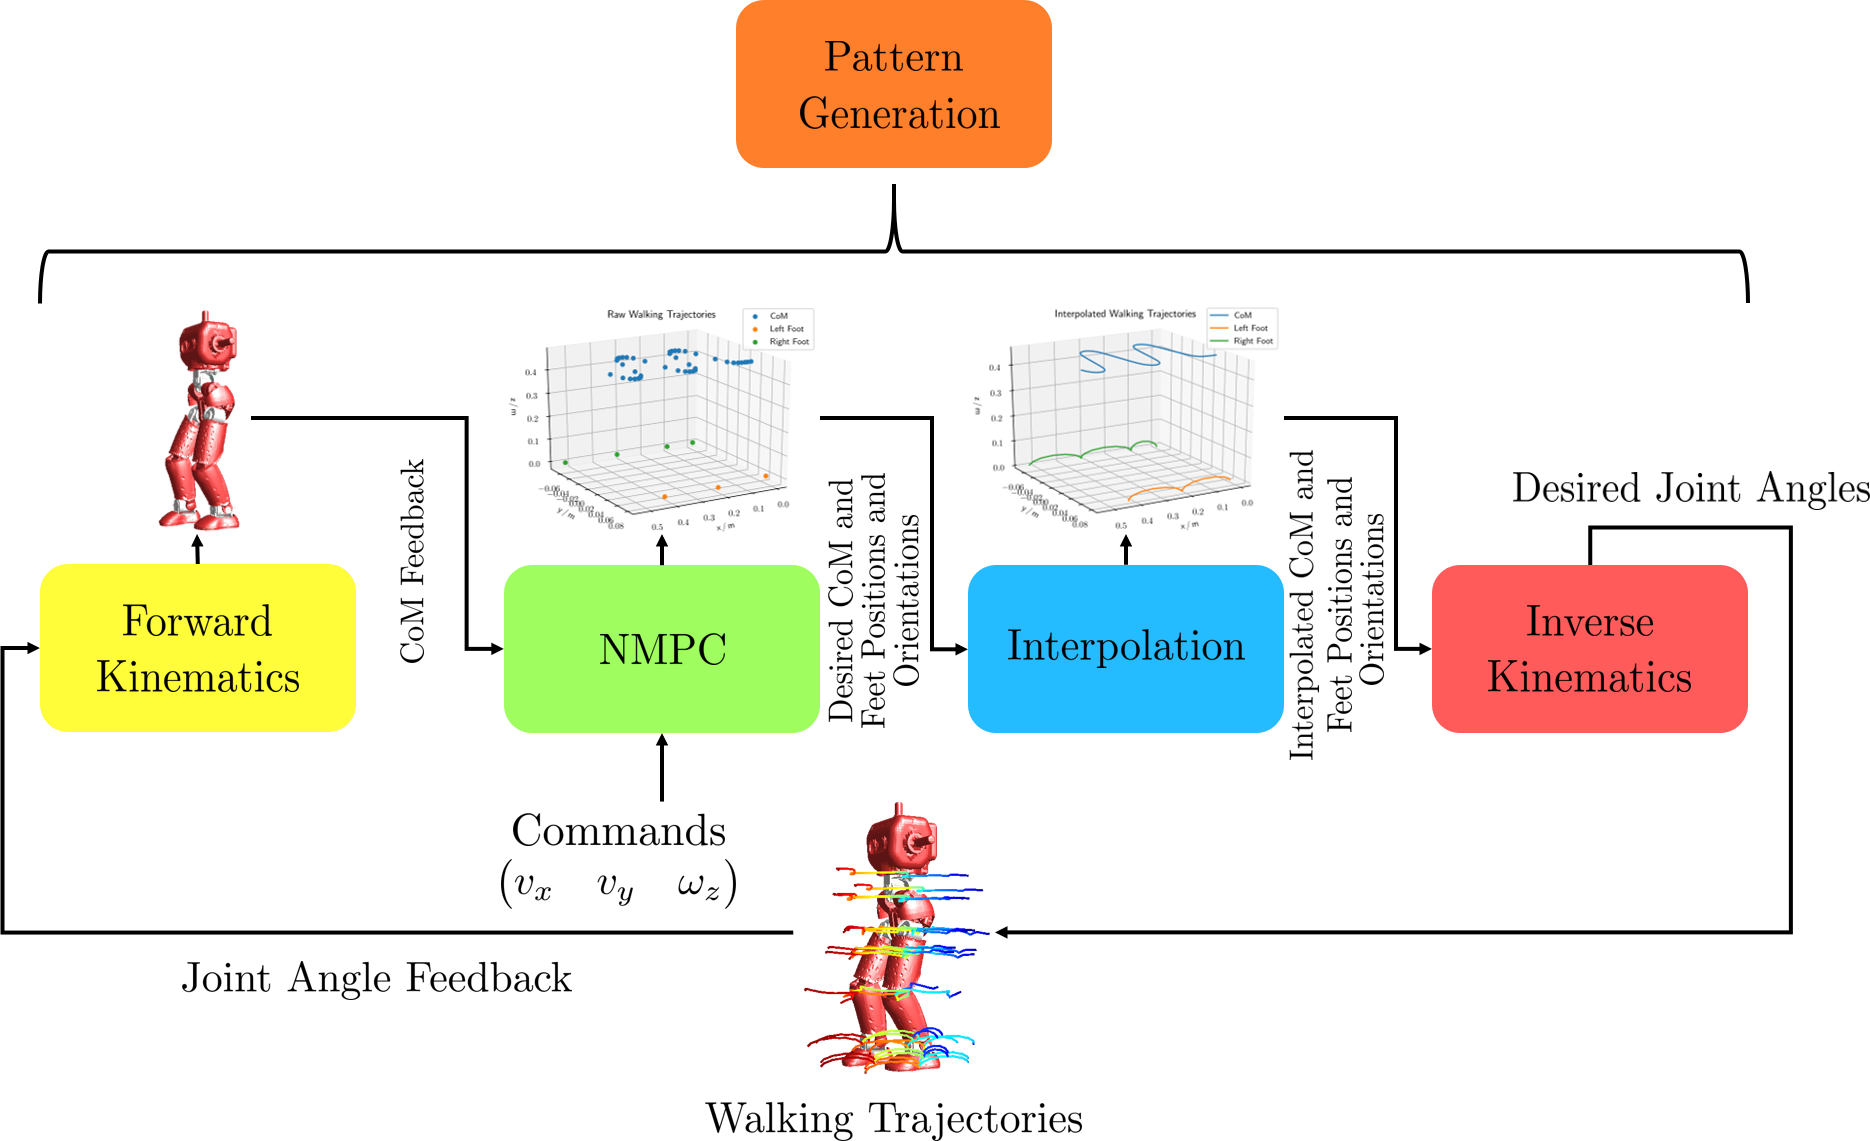
\includegraphics[scale=.5]{chapters/03_background/img/pattern_generation.png}
	\caption{Building blocks of the pattern generation. To understand the greater picture, a connection can be drawn to fig. \ref{fig::3_cl}, where the orange box represents the one shown in this figure.}
	\label{fig::31_pg}
\end{figure}
The natural entry point, to this otherwise closed control loop, is given by the commands that enter the nonlinear model predictive control. Commands are passed in the form of a desired velocity $\mathbf{v}_\text{ref}$ that the robot's center of mass (CoM) shall satisfy optimally according to a cost function that also takes dynamic balance and a smooth motion into account. The future desired positions for the CoM and the feet then result from the solution to a sequentially quadratic problem that tries to minimize this cost function. The balance criteria within this problem formulation is based upon the zero moment point (ZMP) around which the whole control framework is built. It is only by simplifying the robot's model that we can solve the optimal control problem in real time. Therefore, we assume the robot to be a linear inverted pendulum, for which we have a well defined analytical relation between the CoM and the ZMP. The minimization of the distance between the analytical expression of the ZMP and the foot placement results in the desired dynamic balance. As shown in fig. \ref{fig::31_pg}, the desired CoM and the feet positions, as they are obtained from the NMPC, are sparsely distributed in space. Moreover, there is neither information about how the feet shall move along the z-axis, nor along the x-, and y-axis, but only where they should be placed in the x-y-plane. Therefore, as the subsequent step to the NMPC, we need to add an interpolation. The interpolation interpolates the trajectories of the CoM to obtain a finer sampling time. Additionally, the movement of the feet in the x-, y-, and z-direction, as well as their orientation, is computed by polynomials that satisfy the initial and end conditions of the foot placement. 


 